\kapitola{Návrh řešení}
Tato kapitola obsahuje návrh řešení založený na požadavcích identifikovaných v předchozí kapitole. Na základě těchto požadavků byl návrh rozdělen do dvou projektů a to webového frontendu, který slouží jako rozhraní ukazující průběh simulace realném čase a serverové části, která slouží pro rychlý výpočet simulace bez vykreslovaní na platformě Node.js.

Jelikož obě části budou používat stejný simulační kód bylo rozhodnuto, že bude samotná simulace vytvořena jako softwarová knihovna. Tuto závislost ilustruje obrázek \ref{fig:dependency}.
\begin{figure}[h!]
	\centering
	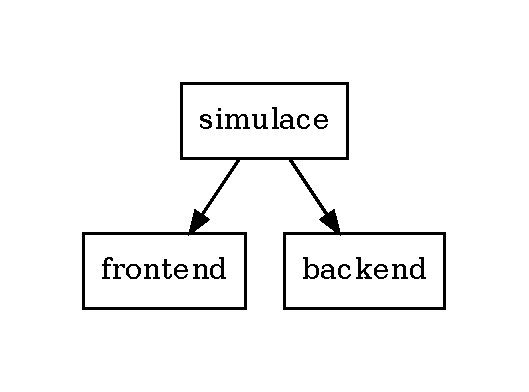
\includegraphics[width=0.4\linewidth]{architektura}
	\caption{Schéma závislostí}
	\label{fig:dependency}
\end{figure}


\sekce{Simulace}
Z obrázku \ref{fig:dependency} je jasné, že simulační kód spojuje obě části dohromady. Je tedy důležité, aby byl navržený tak, aby jej bylo co nejjednodušeji integrovat s oběma řešeními.

Na základě těchto požadavků a podmínek, které jsou stanoveny v předchozí kapitole byl vytvořen následující návrh:

\podsekce{Architektura simulace}

\podsekce{Fitness funkce}
Fitness funkce je důležitou součástí simulace, která zásadně ovlivňuje chování výsledných agentů a je tedy nutné jí volit vhodně. Je nutné, aby funkce agenta motivovala ke správné činnosti.

Po několika pokusech a konzultaci s vedoucím práce byla jako metrika úspěchu agenta zvolena celková vzdálenost, kterou je agent schopný překonat v průběhu jedné generace. Výpočet je realizován s pomocí RoadDirectoru, který si při každém přechodu zaznamená bod, ve kterém se po přesunu agent nachází. Výsledná fitness je pak součet uražených vzdáleností pro každou místnost. Road direktor si pro každou obrazovku uchovává vzdálenost, kterou agent v dané obrazovce překonal. Výsledným fitness je pak součet všech vzdáleností na všech obrazovkách

\sekce{Serverová část}
Serverová část byla nakonec navržena a vytvořena ve dvou na sebe navazujících verzích. 

\podsekce{První verze}
Je ilustrovaná na obrázku \ref{fig:server_first}. Návrh první verze popisuje jednoduchou aplikaci, která rozkládá vyhodnocování jednotlivých genomů mezi jednoho nebo více zpracovatelů. Každý zpracovatel běží ve vlastním vlákně a zátěž je tedy rozložena mezi dostupná jádra procesoru. Zpracovatel po vyhodnocení genomu vrací hlavnímu vláknu fitness daného jedince. Ten si ho uloží a po vyhodnocení všech jedinců tímto způsobem provede algoritmus NEAT. Tento proces se opakuje do té doby, než nedojde k naplnění ukončujících podmínek (maximální počet generací) nebo přerušení programu.

\begin{figure}[h!]
	\centering
	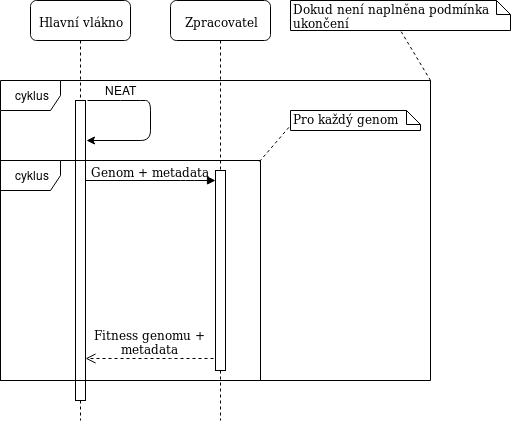
\includegraphics[width=0.7\linewidth]{server_first_use_case}
	\caption{První verze serverové části}
	\label{fig:server_first}
\end{figure}

\podsekce{Druhá verze}
Druhá verze navržená poté, co bylo zjištěno, že předchozí verze nebyla schopná vyhodnotit dostatečné množství genomů dostatečně rychle.

Serverová část pracuje dle diagramu \ref{fig:distributed}, kde je vidět, že klient zadává do fronty úkoly (genom a nastavení simulace). Jednotliví zpracovatelé (počítače v~clusteru), kteří si je z~ní vyberou, jednotlivé genomy vyhodnotí a hodnotu fitness funkce pošlou zpět na klienta. Toto je ilustrováno v diagramu \ref{fig:serverusecase}.

\begin{figure}[h!]
	\centering
	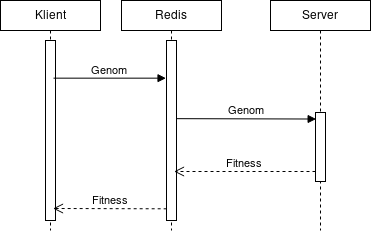
\includegraphics[width=0.7\linewidth]{server_use_case}
	\caption{Sekvenční diagram komunikace se serverem}
	\label{fig:serverusecase}
\end{figure}

Jakmile klient dostane všechny hodnoty zpět provede na populaci genetický algoritmu (mutace, křížení, \dots) a poté je nová generace poslána znovu na vyhodnocení.

\begin{figure}[h!]
	\centering
	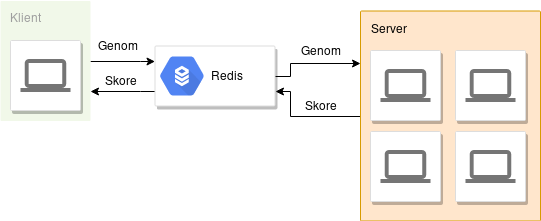
\includegraphics[scale=0.5]{distributed}
	\caption[Schéma distribuovaných výpočtů]{Schéma distribuovaných výpočtů}
	\label{fig:distributed}
\end{figure}

Tento přístup má několik výhod a to:

\begin{enumerate}
	\item Robustnost - Pokud jeden nebo více zpracovatelů selže (je například odpojen ze sítě) je možné pokračovat ve vyhodnocování (neúspěšný úkol lze vrátit zpátky do fronty). Toto v kombinaci s výše zmíněným docker swarmem znamená, že jakýkoliv výpočetní uzel lze kdykoliv vypnout a po znovu zapojení do sítě si načte nejnovější konfiguraci a začne znovu vyhodnocovat bez potřeby jakékoliv manipulace s jakoukoliv částí swarmu.
	\item Dobré rozložení zátěže - Jelikož si zpracovatel vytahuje úkoly z~fronty, je vždy optimálně zatížen, a není třeba řešit rozložení mezi různě výkonnými a zatíženými počítači.
	\item Škálovatelnost - problém lze škálovat až do doby, kdy počet procesorů nepřesáhne počet potřebných simulací. Chceme-li tedy vypočítat generaci o tisíci jedincích můžeme na ně nasadit až tisíc procesorů.
\end{enumerate}

Lze i namítnout, že se zde projevuje určitá režie při síťové komunikaci se serverem, což může být zdrojem určitého zpomalení. Nicméně se toto zpomalení neprojevilo v~průběhu testování clusteru. Právě naopak bylo naměřeno 10 násobné zrychlení oproti výpočtu na jednom počítači.

\podsekce{Databáze}
Všechny verze serverové části zaznamenávají průběh algoritmu NEAT do databáze jejíž schéma lze vidět v obrázku \ref{fig:database}. 
\begin{figure}
	\centering
	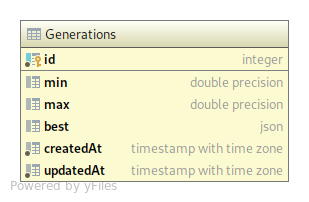
\includegraphics[width=0.7\linewidth]{database}
	\caption{Schéma databáze}
	\label{fig:database}
\end{figure}

